\documentclass{IEEEtran}
\usepackage[utf8]{inputenc}
\usepackage[T1]{fontenc}
\usepackage{amsmath}
\usepackage{amsfonts}
\usepackage{amssymb}
\usepackage{graphicx}
\usepackage{url}
\usepackage{hyperref}
\usepackage[export]{adjustbox}
\usepackage{multicol}

\usepackage[backend=biber]{biblatex}
%\bibliographystyle{ieeetr}
\addbibresource{bibliography.bib}

\usepackage{tikz}
\usetikzlibrary{positioning, arrows}
\tikzset{
block/.style={
  draw, 
  rectangle, 
  minimum height=1.5cm, 
  minimum width=3cm, align=center
  }, 
line/.style={->,>=latex'}
}

\begin{document}

\title{Speech Intelligibility: Detecting Lateral Lisps}
\date{}
\author{\IEEEauthorblockN{Patrick Moritz Samson Munnich}\\
\textit{University of Applied Sciences D\"usseldorf}\\
D\"usseldorf, Germany \\
\href{mailto:patrick.muennich@study.hs-duesseldorf.de}{\texttt{patrick.muennich@study.hs-duesseldorf.de}}}
\maketitle

\section{Abstract}
%Korrektur von Lispeln kann vielen schwer fallen, da ihnen oft nicht bewusst sein kann, ob sie Lispeln oder nicht. Zur Hilfe von Betroffenen haben wir einen Algorithmus zur Identifikation des Sigmatismus Lateralis Lispeln von S-Ger\"auschen in Texten durch Analyse im Frequenzbereich entwickelt. Die Analyse identifiziert Ausschwingungen in gesuchten Frequenzbereichen. Als Frequenzbereiche wurden für das Lispeln 3000-4000\,Hz und für die korrekt Aussprache 2500-3000\,Hz gefunden. Zur Veranschaulichung dessen ist ein Graph von zwei Beispielaufnahmen eines S-Tons mit und ohne Lispeln in Abbildung \ref{examplefft} zu finden. Texte werden in Segmente aufgeteilt und anschließend wird die Analyse auf allen Segmenten ausgeführt. Daraufhin wird verglichen, ob mehr Lispeln oder korrekte Aussprache detektiert wurde. Experimente mit Beispieltexten eines Mannes haben gezeigt, dass die effektivste Segmentlänge bei 0.5\,s liegt und damit 60\% der Texte korrekt eingeteilt werden. In Abbildung \ref{segmentlength} ist die Quote korrekter Detektionen von Textpaaren mit und ohne Lispeln in Abh\"angigkeit der Segmentl\"ange zu sehen. Ein derzeitiges Problem ist, dass inkorrekt eingeteilte Texte konsistent zu häufige Identifikation korrekter Aussprache aufzeigen. Wir hoffen, durch Analyse weiterer Stimmen und Weiterentwicklung des Algorithmus, insbesondere der Identifikation korrekter Aussprache, die Ergebnisse weiter verbessern zu können.

Correcting lisps can prove to be of great difficulty to many,
as they may be unaware of whether they are lisping.
To help those affected,
we have developed an algorithm for identification of the sigmatismus lateralis in ''S'' sounds within speech recordings via analysis in the frequency domain.
The algorithm identifies peaks within the lisp's frequency band after calibration.
We have generally identified a frequency band of 3000-4000\,Hz to be generally accurate for the lisp and 2500-3000\,Hz for the correct pronunciation.
Our algorithm splits given files into smaller segments and compares the number of lisps and non-lisps detected in these segments to categorize the file.
From tests,
we concluded that a segment length of 0.5\,s produces the best results.
The algorithm was able to detect 60\% of our tested pairs of lisped and non-lisped pronunciations of the same text properly.
Our implementation in Julia with multi-threaded per-file analysis is able to analyze 20 files of lengths between 5\,s and 10\,s within 2.5\,s on an AMD Ryzen 3700x,
with 98\% of the time spent on compilation,
meaning analysis is far faster than real-time.
The algorithm itself should be easily expanded to identify other sounds,
e.g.\ other kinds of lisps.

\section{Introduction}

Lisps are functional speech disorders characterized by difficulties in pronouncing sibilants such as 's' or 'z' properly.
A common variant of this is the lateral lisp,
sigmatismus lateralis (SL),
where a person produces sibilants using the side of their mouth instead of the front,
often by blocking their front teeth with their tongue,
forcing air out the sides of their mouth.
A visualization of this specific lisp compared to a proper sibilant production is in fig.\ \ref{lispvisual},
where the arrows point in the direction of air flow.

\begin{figure}[h]
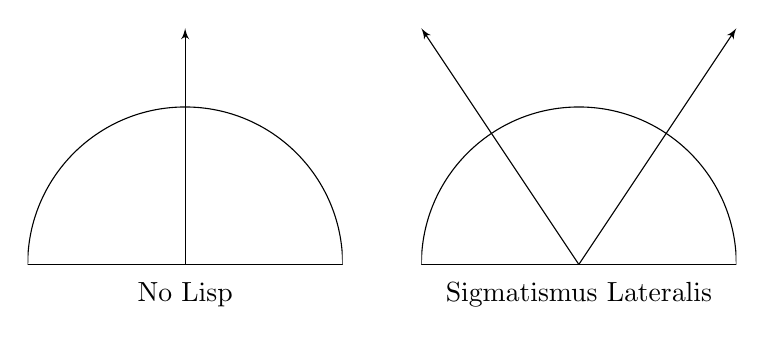
\begin{tikzpicture}[baseline=(current bounding box.north)]
\begin{scope}
    \clip (-2,0) rectangle (2,2);
    \draw (0,0) circle(2);
    \draw (-2,0) -- (2,0);
\end{scope}
\draw[line] (0,0) -> (0,3);
\begin{scope}
    \clip (3,0) rectangle (7,2);
    \draw (5,0) circle(2);
    \draw (3,0) -- (7,0);
\end{scope}
\draw[line] (5,0) -> (7,3);
\draw[line] (5,0) -> (3,3);
\node[below= 1mm of {(0,0)}] {No Lisp};
\node[below= 1mm of {(5,0)}] {Sigmatismus Lateralis};
\end{tikzpicture}
\caption{Comparison of sibilant production without an SL (left) and with an SL (right). 
The arrows point in the direction of air flow;
a standard sibilant production moves air out the front,
while an SL moves air out one or both sides of the mouth.}\label{lispvisual}
\end{figure}

Noticing whether one is lisping can be difficult,
especially in early stages of the correction process.
As such,
it is our goal to develop a simple and fast algorithm that can potentially be run in real-time on a weak device such a smartphone.

Similar research includes detecting sibilants for suppression of loud hissing in recordings \cite{Gonzalez} \cite{de-ess} and replacement of lisps in text-to-speech software using Random Forest Classifiers \cite{Itagi}.
However,
these are not tailored towards the SL,
nor are the lightweight enough to be ran in real-time on weaker devices.

\section{Proposed Method}

\subsection{Analyzing a single case}\label{analyze}

To analyze a single case of the SL,
we use a male test subject with previous experience with the speech impediment.
We use the following parameters for our recordings:

\begin{itemize}
	\item Bit depth: 16-bit
	\item Sampling frequency: \(f_\mathrm{s} = 8000\)\,Hz
	\item Length of recording: \(t = 5\)\,s
	\item Number of recordings: 6
	\item Microphone: Gyvazla SML
\end{itemize}

Both SL and normal S sounds (S) are recorded with no pauses or other sounds.
These recordings are then split into segments of 8000 samples (\(t = 1\)\,s),
over which we run a fast Fourier transform (FFT) algorithm.
To analyze these segments, we plot the absolute of the FFT and find consistent peaks around 2500-3000\,Hz for the S and 3000-4000\,Hz for the SL.
One such comparison graph can be scene in fig.\ \ref{examplefft}.

\begin{figure}[h]
\centering
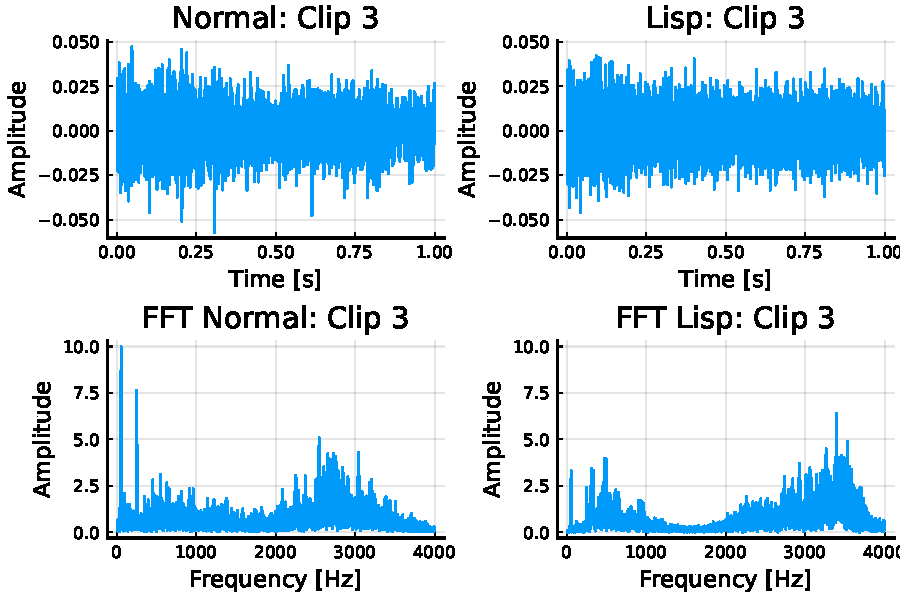
\includegraphics[trim=0 0 0 145, clip, scale=0.55]{normal_vs_lisp_clip_3.pdf}
\caption{Comparison of two recordings of S (left) and SL (right) in the frequency domain. Clear peaks are visible around 2500-3000\,Hz for S and 3000-3500\,Hz for SL. Additional peaks that the human voice cannot have produced are visible below 1000\,Hz.}\label{examplefft}
\end{figure}

\subsection{Identification algorithm}\label{identify}

To identify which sound we're dealing with,
we begin by again splitting into aforementioned segments of 8000 samples each.
For these, we subtract our recording's mean and normalize in order to account for varying volumes.
We again must calculate the absolute of the FFT of the segment we want to analyze.
In order to remove unwanted low frequencies not made by the test subject,
we apply a high pass filter as described in eq.\ \ref{highpass} with boundary \(b = 1000\)\,Hz.

\begin{equation}
H(x, b) = \begin{cases} x\ \mathrm{for}\ x < b \\ 0\ \mathrm{else} \end{cases}\label{highpass}
\end{equation}

Frequencies below 1000\,Hz showed numerous minor peaks in tests,
which are not typical of sibilants and are discarded.
These peaks are also visible in fig.\ \ref{examplefft}.

Past this boundary, we assume a noise floor to be present.
This noise floor will later be used to detect the peaks for S and SL.
To again compensate for variations, we normalize the FFT magnitudes.

With our FFT magnitudes prepared for analysis,
we can now use the peak bands found in \ref{analyze} of 2500-3000\,Hz for S and 3000-4000\,Hz for SL.
We separate our magnitudes into the band we want to analyze and the rest of the frequencies,
for which we calculate the arithmetic mean and compare.
If the band's mean is greater than the rest's,
we assume the band's sound to be present.

A flow diagram of this algorithm can be found in fig.\ \ref{examinesegment}

\begin{figure}[h]
\centering
\scalebox{0.45}{
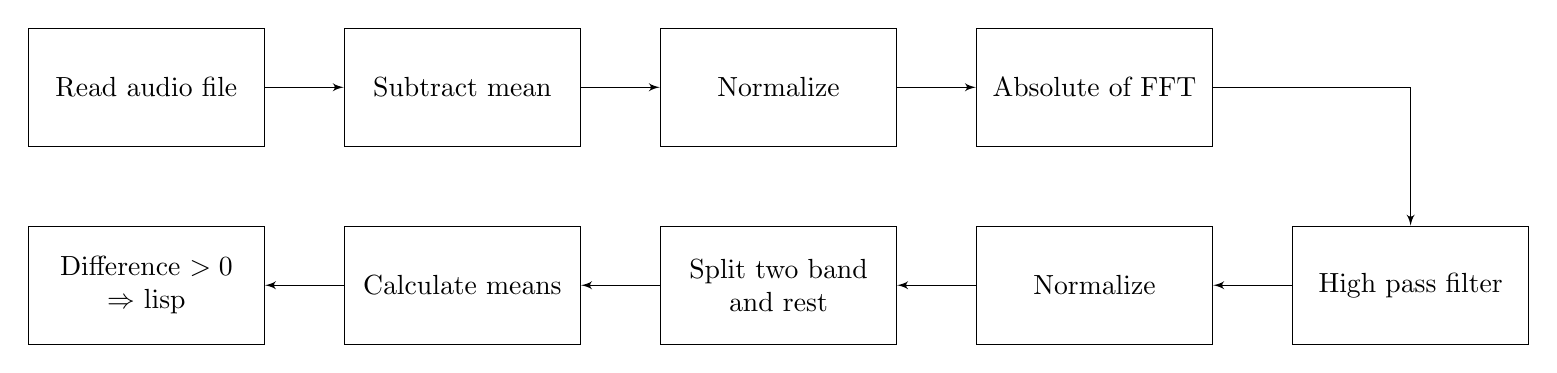
\begin{tikzpicture}

\node[block]	(read)														{Read audio file};
\node[block]	(subtraction)	[right=of read]								{Subtract mean};
\node[block]	(normalizesub)	[right=of subtraction]						{Normalize};
\node[block]	(absfft)			[right=of normalizesub]						{Absolute of FFT};
\node[block]	(slice)			[below right=1cm and 1cm of absfft]			{High pass filter};
\node[block]	(normalizefft)	[left=of slice]								{Normalize};
\node[block]	(split)			[left=of normalizefft]						{Split two band \\ and rest};
\node[block]	(mean)			[left=of split]								{Calculate means};
\node[block]	(thresh)			[left=of mean]								{Difference $> 0$ \\ $\Rightarrow$ lisp};

\draw[line] 	(read.east) 		-- 	(subtraction.west);
\draw[line]	(subtraction.east) 	--	(normalizesub.west);
\draw[line] 	(normalizesub.east) 	--	(absfft.west);
\draw[line] 	(absfft.east) 		-|	(slice.north);
\draw[line] 	(slice.west)			--	(normalizefft.east);
\draw[line] 	(normalizefft.west) 	-- 	(split.east);
\draw[line] 	(split.west)			--	(mean.east);
\draw[line] 	(mean.west) 			-- 	(thresh.east);
\end{tikzpicture}
}
\caption{Flow diagram for identification of S and SL in recordings.}\label{examinesegment}
\end{figure}

\subsection{Calibration for other test subjects}

As the lisp detection can easily fail for other subjects due to e.g.\ differing voice pitches,
slight differences in lisping methods, or differing microphones,
a calibration is necessary for the algorithm to perform properly.

To achieve this,
we run a simple algorithm to detect the desired range.
First, we run the same high-pass pass filter as before with the same boundary \(b = 1000\)\,Hz.
We use a peak finding algorithm forked from \cite{findpeaks} that works by comparing the height of the amplitude to a threshold \(h_\mathrm{min}\) calculated applying eq.\ \ref{hmin} on the absolute of the FFT \(A\):

\begin{equation}
h_\mathrm{min} = \frac{\max(A)}{4}
\label{hmin}
\end{equation}

We then filter out all the peaks the algorithm finds which are more than 1000\,Hz from another peak.
The resulting range for the example in fig.\ \ref{examplefft} is 2250-3249\,Hz for S and 2788-3784\,Hz for SL,
roughly coinciding with the previously used frequency ranges.
A visualization of these results for the aforementioned example can be found in fig.\ \ref{examplecalibration}.

\begin{figure}[h]
\centering
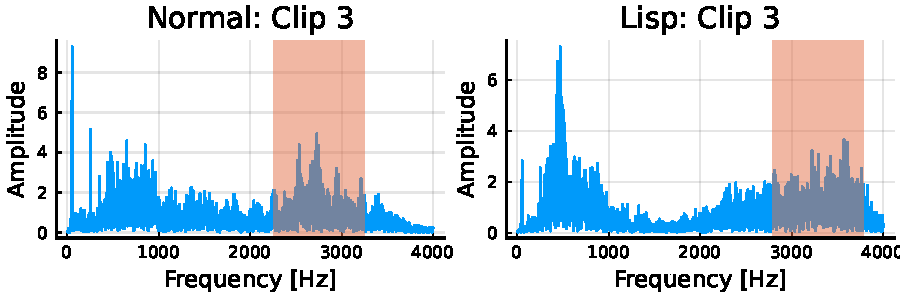
\includegraphics[scale=0.55]{calibration.pdf}
\caption{Comparison of two recordings of S (left) and SL (right) in the frequency domain with calibration algorithm's detected prominent ranges highlighted.}\label{examplecalibration}
\end{figure}

\subsection{Adjustment to full texts}

To extend the algorithm from \ref{identify} so it can be used to analyze full texts,
we use a similar setup as in \ref{analyze} with texts of length \(t = 5\)\,s once with and once without an SL.
These recordings are split into smaller segments and their arithmetic means are compared with the full audio file's.
Segments with lower means are considered silent or too noisy and discarded.
Our algorithm is then run over the remaining segments for both the S and SL ranges and the number of matches for the audio file are counted.
We then compare which range had a larger number of matches,
indicating whether the S or SL was present.

To find an ideal segment length,
10 recordings were tested with differing segment lengths between 0.1\,s and 1.0\,s in steps of 0.15\,s for one test subject and the results compared.
The most accurate results were achieved with a segment length of 0.5\,s with 60\% of pairs correctly assigned as S and SL.
Lower values rapidly fell in accuracy,
while higher values stagnated at around 20\% lower accuracy.
A graph of the results is in fig.\ \ref{segmentlength}

\begin{figure}[h]
\centering
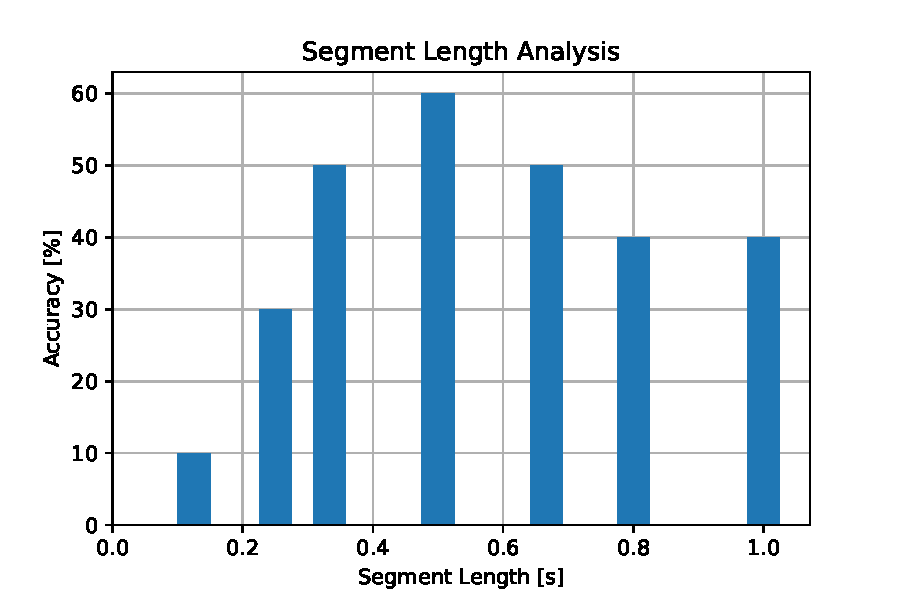
\includegraphics[scale=0.5]{seglen.pdf}
\caption{Detection algorithm's accuracy for pairs of S and SL texts for different segment lengths. A clear peak can be seen at 0.5\,s, indicating this might be the ideal segment length.}\label{segmentlength}
\end{figure}

\section{Results}

\section{Conclusion}

\nocite{*}

\printbibliography


\end{document}